%% ceci est un commentaire 
%% il faut toujours commencer par \documentclass[type de papier, taille de texte]{sytle du document}
\documentclass[a4paper,10pt]{report} %%%% sytle du document : report/book/article


%%%%%%%%%%%%%%%%%%%%%%%%%%%%%%%%%%%%%%%%%%%%%%%%%%%%%%%%%%%%%%%%%%%%%%%%%%%%%%%
%% la suite est une collection des "package" ou des "librararies" pour utiliser des codes spécifiques

%% il vous suffit de les copie-coller quand vous créez un nouveau document TeX (ou bien en ajouter plus si besoin).
\usepackage[utf8]{inputenc} %% pour les accents en français
\usepackage[frenchb]{babel} %% pour un format français
\usepackage{graphicx} %% pour afficher des graphiques
\usepackage{amsmath} %% pour écrire des symboles (maths), des équations, etc.
\usepackage{amssymb}
\usepackage{color}
\usepackage{bm} %% pour lister des citations/la biblio
\usepackage{hyperref} %% pour inserer des liens internet
\usepackage{cleveref} %% pour faire des références uax équations, tableaux, etc.
\usepackage{cite}
\usepackage{float}
%\usepackage{setspace} %% pour changer l'espace entre les lignes
%\linespread{1.6} %% pour changer l'espace entre les lignes



%%%%%%%%%%%%%%%%%%%%%%%%%%%%%%%%%%%%%%%%%%%%%%%%%
% Default fixed font does not support bold face
\DeclareFixedFont{\ttb}{T1}{txtt}{bx}{n}{8} % for bold
\DeclareFixedFont{\ttm}{T1}{txtt}{m}{n}{8}  % for normal

% Custom colors
\usepackage{color}
\definecolor{deepblue}{rgb}{0,0,0.5}
\definecolor{deepred}{rgb}{0.6,0,0}
\definecolor{deepgreen}{rgb}{0,0.5,0}

\usepackage{listings}

% Python style for highlighting
\newcommand\pythonstyle{\lstset{
language=Python,
breaklines=true,
basicstyle=\ttm,
otherkeywords={self},             % Add keywords here
keywordstyle=\ttb\color{deepblue},
emph={MyClass,__init__},          % Custom highlighting
emphstyle=\ttb\color{deepred},    % Custom highlighting style
stringstyle=\color{deepgreen},
frame=tb,                         % Any extra options here
showstringspaces=false 
           % 
}}


% Python environment
\lstnewenvironment{python}[1][]
{
\pythonstyle
\lstset{#1}
}
{}

% Python for external files
\newcommand\pythonexternal[2][]{{
\pythonstyle
\lstinputlisting[#1]{#2}}}

% Python for inline
\newcommand\pythoninline[1]{{\pythonstyle\lstinline!#1!}}







%%%%%%%%%%%%%%%%%%%%%%%%%%%%%%%%%%%%%%%%%%%%%%%%%%%%%%%%%%%%%%%%%%%%%%%%%%%%%%%
\title{------ Vabiration Libres d'une Poutre en Flexion ------} %% choissez un titre approprié à votre sujet
\author{par\\GAYE, Ibrahima\\ ZHANG, Xunjie\\ Compte-rendu du Ex.31 de l'UE Outil de Mathématique } %% utilisez \\ pour une nouvelle ligne
\date{fait le 28 octobre 2016} %% pour afficher la date actuelle commenter cette ligne








%%%%%%%%%%%%%%%%%%%%%%%%%%%%%%%%%%%%%%%%%%%%%%%%%%%%%%%%%%%%%%%%%%%%%%%%%%%%%%%
%% TOUT ce qui va dans votre rapport doit être entre \begin{document} & \end{document}
\begin{document}
\selectlanguage{french} %% format français
\maketitle %% pour afficher le titre
\tableofcontents %% pour afficher/compiler le sommaire automatiquement
\listoffigures %% pour lister les figures













%%%%%%%%%%%%%%%%%%%%%%%%%%%%%%%%%%%%%%%%%%%%%%%%%%%%%%%%%%%%%%%%%%%%%%%%%%%%%%%
\chapter{Introduction et Séparation des variables}

\section{Introduction}

On ne traitera que ici que le probléme d'une poutre droite , de section uniforme , en flexion simple dqns un plan principal .
Ce pendant , le plus souvent , la poutre n'est pas contrainte à rester dans ce plan , et il existe une possibilité de déplacement dans la direction perpendiculaire . Si les excitations ne sont pas contenues dans un plan principal , il faut étudier les virations de flexion , dans les 2 plans principaux définis chacun par l'axe de la poutre et l'une des directions principales de la section .


\section{Séparation des variables}

\subsection{Équation d'Équilibre}

Pour une poutre droite de section constante en flexion , et considérons un effort extérieur $t_{ext}$ nul , on a l'équation :
\begin{equation}
    \frac{\partial^2v}{\partial{v}^2}=-\frac{El}{\rho S}\frac{\partial^4{v}}{\partial{x}^4}
	\label{equantion1}
\end{equation}


Posons : $v(x,t)$=$\phi(x)q(t)$ et reportons cette expression dans l'équation du mouvement :
\begin{equation}
	\phi\frac{d^2{q}}{d{t}^2}=-\frac{El}{\rho S}\frac{d^4{\phi}}{d{x}^4}q
	\label{equantion2}
\end{equation}


\subsection{Séparations}
Séparons les termes qui dépendent de $t$ et de $x$ :
\begin{equation}
    \frac{1}{q}\frac{d^2{q}}{d{t}^2}=-\frac{El}{\rho S}\frac{d^4{\phi}}{d{x}^4}\frac{1}{\phi}
    \label{equantion3}
\end{equation}

%%%%%%%%%%%%%%===================%%%%%%%%%%%%%%%%%%%%%%%ù
\section{Solution des fonctions}

Les 2 membres de cette équation sont indépendants l'un de x , l'autre de t ; ils sont donc constants . Pour que la solution$q(t)$ reste bornée quand le temps tend vers l'infini , cette valeur constante doit être négative .
\begin{center}
Trouver $q(t)$ et $\phi(x)$ quand $-\omega^2$ est constant :
	\begin{equation}
		\frac{1}{q}\frac{d^2{q}}{d{t}^2}=-\frac{El}{\rho S}\frac{d^4{\phi}}{d{x}^4}\frac{1}{\phi}=-\omega^2
		\label{equation4}
	\end{equation}
\end{center}


\subsection{équation différentielles ordinaires}

On en tire 2 équations différentielles ordinaires , l'une en $x$ , l'autre en $t$ , que l'on résout séparément :
\begin{equation}
	\left\{
    \begin{array}{r c l }
        \frac{d^4\phi}{dx^4}-\omega^4\frac{\rho S}{EI}\phi&=&0\\
        \frac{d^2q}{dt^2}+\omega^2 q&=&0
    \end{array}
    \right.
\end{equation}
%%%%%=====================================%%%%%%%%%%%%%
\subsection{recherche la solution}

On recherche la solution de l'équation sous la forme harmitienne suivante :
   $\phi (x)=ae^{sx}$ , d'où léquation caractéristique , de degré 4 en $S$ :

\begin{equation}
	s^4-\omega^4\frac{\rho S}{EI}=0
	\label{equation5}
\end{equation}

qui a solutions :

\begin{equation}
    s=\pm \sqrt[4]{\frac{\rho S}{EI}{\omega^2}}\ ,\ s=\pm i\sqrt[4]{\frac{\rho S}{EI}{\omega^2}}
    \label{equation6}
\end{equation}

que l'on peut aussi écrire en fonction d'unparamètre $\gamma$ sans dimension :

\begin{equation}
    s=\pm\frac{\gamma}{L}\ ,\ s=\pm i\frac{\gamma}{L}\ , \gamma=L\sqrt[4]{\frac{\rho S}{EI}{\omega^2}}
    \label{equation7}
\end{equation}


On en déduit l'expression de la forme modale :

\begin{equation}
    \phi (x)=ae^{\gamma\frac{x}{L}}+be^{-\gamma\frac{x}{L}}+ce^{i\gamma\frac{x}{L}}+de^{-i\gamma\frac{x}{L}} 
    \label{equation8}
\end{equation}

ou encore :


\begin{equation}
    \phi (x)=A\sinh{(\gamma\frac{x}{L})}+B\cosh{(\gamma\frac{x}{L})}+C\sin{(\gamma\frac{x}{L})}+D\cos{(\gamma\frac{x}{L})}
    \label{equation9}
\end{equation}

On recherche l'autre solution de l'équation sous la forme harmitienne suivante : 
$q(t)=ae^{bx}$ , d'où léquation caractéristique , de degré 2 en $t$ :

\begin{equation}
    b^2+\omega^2=0
    \label{equation10}
\end{equation}

qui a 2 solutions :

\begin{equation}
    b=\pm i\omega\ , \ \omega=\frac{\gamma^2}{L^2}\sqrt{\frac{EI}{\rho S}}
    \label{equation11}
\end{equation}

Donc on en déduit l'expression de la forme modale :

\begin{equation}
    q(t)=\hat{e}e^{i\omega t}+\hat{f}e^{-i\omega t}
    \label{equation12}
\end{equation}

Ou encore :

\begin{equation}
    q(t)=E\sin{\omega t}+F\cos{\omega t}\ , \ \omega=\frac{\gamma^2}{L^2}\sqrt{\frac{EI}{\rho S}}
    \label{equation13}
\end{equation}


\section{Solution finalement}
On obtient donc finalement :
\begin{equation}
	v(x,t)=\phi (x)q(t)
	\label{equation15}
\end{equation}

avec:
\begin{equation}
    \left\{
    \begin{array}{r c l}
        \phi(x)&=&A\sinh(\gamma\frac{x}{L})+B\cosh(\gamma\frac{x}{L})+C\sin(\gamma\frac{x}{L})+D\cos(\gamma\frac{x}{L})\\q(t)&=&E\sin{\omega t}+F\cos{\omega t}\\
        \omega&=&\frac{\gamma^2}{L^2}\sqrt{\frac{EI}{\rho S}}
    \end{array}
    \right.
\end{equation}

\begin{itemize}
    \item $\phi (x)$  définit la form de la poutre pendant sa vibration . Elle contient les 5 constantes $A, B, C$ et $\gamma (ou\ \omega)$ , qui sont fixées par les conditions aux limites .
    
    \item $q(t)$ définit le mouvement de la poutre . Elle contient , outre la constante $\omega$ déjà évoquée , les 2 constantes $E$ et $F$ , qui sont fixées par les conditions initiales .
\end{itemize}



%%%%%%%%%%%%%%%%%%%%%%%%%%%%%%%%%%%%%%%%%%%%%%%%%%%%%%%%%%%%%%%%%%%%%%%%%%%%%%%%%%%%%%%%%%%%
\chapter{Résolution dans le cas de la poutre encastrée-appuie} %% pour commencer un chapitre


%%%%%%%%%%%%%%%%%%%===============%%%%%%%%%%%%
\section{conditons limites}

Il existe 2 conditions aux limites usuelles pour une poutre en flexion :

\subsection{extrémité en appui simple à l'abscisse x=L}

La flèche esy nulle en tout instant , ainsi que le moment fléchissant :

\begin{equation}
    \forall t\, 
    \left\{
    \begin{array}{r c l}v(L,t)&=&0\\\frac{\partial ^2v}{\partial x^2}(L,t)&=&0
    \end{array}
    \right.
\end{equation}

On a :

\begin{equation}
    \left\{
    \begin{array}{r c l}
    \phi (L)&=&A\sinh{\gamma}+B\cosh{\gamma}+C\sin{\gamma}+D\cos{\gamma}=0\\
    \frac{d^2\phi}{dx^2}(L)&=&\frac{\gamma^2}{L^2}A\sinh{\gamma}+B\frac{\gamma^2}{L^2}\cosh{\gamma}-C\frac{\gamma^2}{L^2}\sin{\gamma}-D\frac{\gamma^2}{L^2}\cos{\gamma}=0
    \end{array}
    \right.
\end{equation}

Et on en déduit :

\begin{equation}
    \left \{
    \begin{array}{r c l}
    A\sinh{\gamma}+B\cosh{\gamma}&=&0\\
    C\sin{\gamma}+D\cos{\gamma}&=&0
    \end{array}
    \right.
\end{equation}

\subsection{Encastrement à l'abscisse x=0}

La flèche esy nulle en tout instant , ainsi que la pent de la poutre : 

\begin{equation}
    \forall t\,
    \left \{
    \begin{array}{r c l}v(0,t)&=&0\\\frac{\partial v}{\partial x}(0,t)&=&0
    \end{array}
    \right.
\end{equation}

d'où , on a :

\begin{equation}
    \left\{
    \begin{array}{r c l}
    \phi (0)&=&B+D=0\\\frac{d\phi}{dx}(0)&=&A\frac{\gamma}{L}+C\frac{\gamma}{L}=0
    \end{array}
    \right.
\end{equation}

On en déduit :

\begin{equation}
    \left\{
    \begin{array}{r c l}
    A+C&=&0\\
    B+D&=&0
    \end{array}
    \right.
\end{equation}


\subsection{Résultat par les conditions limites}

On cherche solution pour les 4 équations :
\begin{equation}
    \left\{
    \begin{array}{r c l}
    &A\sinh{\gamma}+B\cosh{\gamma}=0\\
    &C\sin{\gamma}+D\cos{\gamma}=0\\
    &A+C=0\\
    &B+D=0
    \end{array}
    \right.
\end{equation}

On trouve simplement:


\begin{equation}
    \left\{
    \begin{array}{r c l}
    &\tanh{\gamma}-\tan{\gamma}=0\\
    &B=-A\tanh{\gamma}=-A\tan{\gamma}
    \end{array}
    \right.
\end{equation}

%%%%%%%%%%%%%========%%%%%%%%%%%%%%
\section{Infinité de solutions}

On écrit une programme pour trouver les n valeurs , ce que on noté $\gamma_n$ , et un tracé graphique simple permet d'apprecher les solutions . En effect , l'équation peut s'écrire :


\begin{equation}
    \tanh{\gamma}=\tan{\gamma}
\end{equation}

Les solutions sont données par les intersections des courbes $\tanh{\gamma}$ et $\tan{\gamma}$:

\begin{figure}[H]
\centering
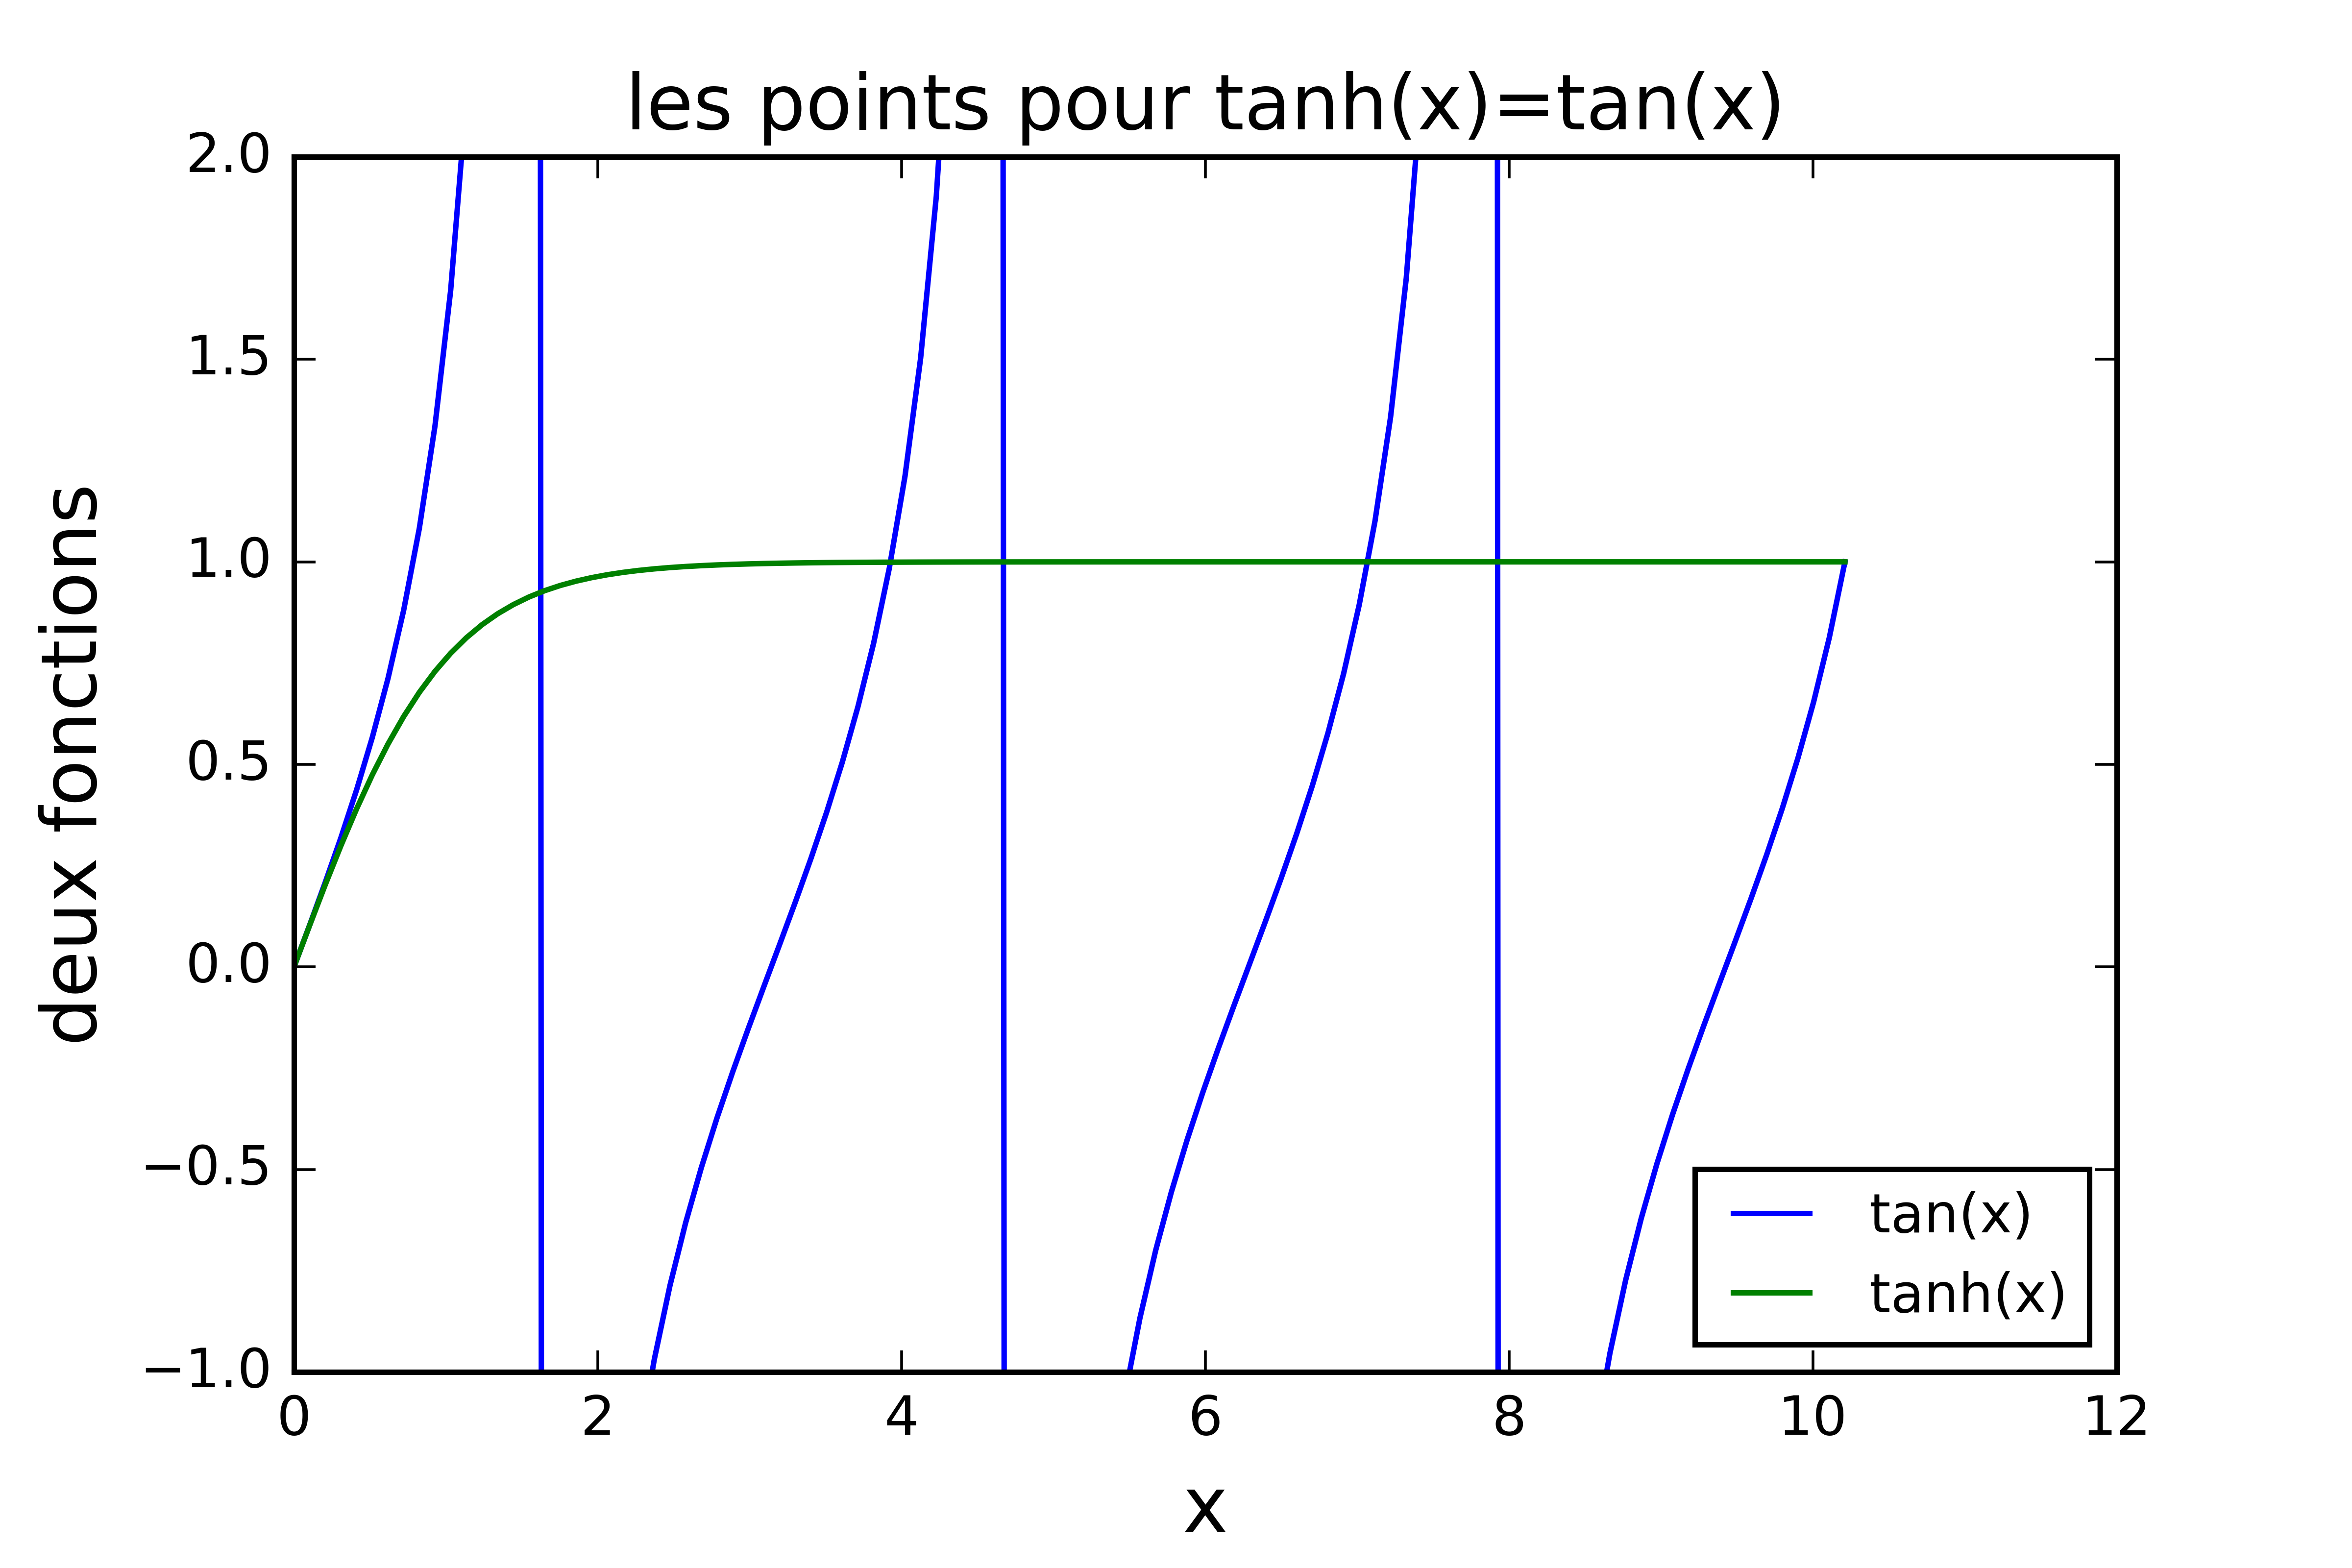
\includegraphics[width=1.0\textwidth]{figuretanh}
\caption{infinité points}
\label{figure1}
\end{figure}

On constate qu'il esixste une infinité de solution , voisines de $\frac{9\pi}{4},\frac{13\pi}{4},\frac{5\pi}{4}$ , etc.
Les valeurs précises peuvent être 
















La construction de la matrice $A$ et du vecteur $B$ se font de manière relativement simple. En effet, nous devons calculer $A^k$ et $B^k$ pour chaque élément, puis les assembler, avant de résoudre le système.
La façon la plus simple est de remplir $A$ $B$, en incrémentant la valeur de $k$.

En retrouve cette forme:

$$A^k =\begin{bmatrix}
A^k_11 + A^{k-1}_22 & A^k_12 \\
A^k_12 & A^k_22 + A^{k+1}_11
\end{bmatrix}, k \neq 0, k \neq N$$

On tiendra compte des valeurs limites et de la particularité des valeurs de $A^1_{11}$,$B^1_{11}$ et $B^N_{12}$ qui ne requière pas d'addition avec des valeurs voisines.
Une fois le système implémenté, sa résolution et la comparaison avec les valeurs analytique seront relativement simples.

\section{Programme}

Le programme se décompose en trois parties. Nous avons d'abord défini les fonctions qui nous permettront de construire notre système, ainsi que la solution analytique. Puis, nous avons étudié la solution approchée pour des paramètres donnée et avec un maillage avec 5 éléments ($N=5$).Nous avons terminé le programme avec une étude de l'erreur relative en un point donné en fonction de la variation du nombre de nœuds.

Le programme fonctionne très bien et est joint en annexe. Il sauvegarde automatiquement les courbes tracées.


%%%%%%%%%%%%%%%%%%%%%%%%%%%%%%%%%%%%%%%%%%%%%%%%%%%%%%%%%%%%%%%%%%%%%%%%%%%%%%%

\chapter{Résultats et Conclusions}

\section{Résultats}
 
\subsection{Solution approchée pour N=5}

\subsubsection{Courbe approchée}
\begin{figure}[H]
\begin{center}
%	\includegraphics[width=0.7\textwidth]{{"FIG/U Uh N5"}.png}
\end{center}
\caption{Solution approchée pour $N=5$}
\label{U Uh N5}
\end{figure}
Les valeurs sont de l'ordre de grandeur des déplacements possibles dans nos modèles physiques connues.
On remarque très bien que les valeurs trouvées numériquement sont très proches de celle de la courbe analytique en rouge. On peut aussi voir que si on fait une interpolation polynomiale d'ordre 1, c'est-à-dire relier tous les points bleus par des droites, la forme de la solution approchée sur des valeurs autre que celle des nœuds reste inexacte et ne correspond pas à la forme de la solution analytique.


\subsubsection{Erreur relative en chaque nœud}
\begin{figure}[H]
\begin{center}
	%\includegraphics[width=0.7\textwidth]{{"FIG/Erreur relative N5"}.png}
\end{center}
\caption{Erreur relative en chaque nœud pour $N=5$}
\label{Erreur relative N5}
\end{figure}


Sur chaque nœud, nous avons calculé l'erreur relative de la solution approchée  $$Err = \frac{||u-u_{h}||}{||u||}$$
On remarque qu'elle est très faible et qu'elle diminue légèrement en fonction de $r$. On voit aussi que pour le premier nœud, ou $r=0$, nous avons un écart important, même si les valeurs des solutions analytique et approchée tendent vers $0$. Cette erreur numérique est due au fait que l'erreur relative ne peut être calculée en ce point. Ce que nous avons sont des valeurs très proches de $0$, mais non nulles que l'ordinateur calcul quand même. On peut ne pas tenir compte de cet effet de bord.

\subsection{Étude pour N croissant}
\subsubsection{Solutions Approchées}
\begin{figure}[H]
\begin{center}
	%\includegraphics[width=0.7\textwidth]{{"FIG/Solutions Approchees & Analytique"}.png}
\end{center}
\caption{Solutions Approchées pour un nombre de nœud croissant}
\label{SANcroissant}
\end{figure}

On remarque que très rapidement, les courbes des solutions approchées se confondent avec la courbe de la solution analytique. On peut déjà prétendre que la solution approchée converge vers la solution exacte quand le nombre de nœuds augmente.

\subsubsection{Erreur relative}
\begin{figure}[H]
\begin{center}
	%\includegraphics[width=0.7\textwidth]{{"FIG/Erreur relative fct de h"}.png}
\end{center}
\caption{Évolution de l'erreur relative en fonction de la finesse du maillage $h$}
\label{Erreur relative fct de h}
\end{figure}

\begin{figure}[H]
\begin{center}
	%\includegraphics[width=0.7\textwidth]{{"FIG/Erreur relative fct de N"}.png}
\end{center}
\caption{Évolution de l'erreur relative en fonction du nombre de nœuds $h$}
\label{Erreur relative fct de N}
\end{figure}

Dans cette partie nous avons calculé et tracé l'erreur relative en fonction de l'évolution de $h$. L'erreur relative a été calculée au nœud $r_{n}=L$, à l'extrémité de la pale.
On remarque que l'erreur diminue si la finesse du maillage augmente. Cette diminution n'est pas linéaire. On peut en déduire qu'à partir d'un certain seuil, l'augmentation de la finesse ne sera plus intéressante d'un point de vue numérique. En effet, en augmentant le maillage, nous augmentons les efforts de calcul de la machine. À partir d'un certain seuil, le gain en précision devient négligeable, comme la courbe tend vers zéro.
Se pose alors la question de la capacité et la durée du calcul fait par la machine. Cette durée est aussi dépendante de la complexité du calcul, dans les cas en $2D$ et $3D$. 




\subsection{Influence du polynôme d'interpolation}

Malheureusement, par manque de temps, nous n'avons pas pu tester avec une interpolation polynomiale de degré 2. La solution approchée aurait était plus proche de la solution analytique, notamment par le fait que le nombre de nœuds augmente dans ce cadre.
Nous n'avons pas non-plus étudié l'erreur relative en tout point $x$. Cette erreur est plus importante entre deux nœud. En l'étudiant, nous aurions pu comparer l'influence du polynôme d'interpolation dans l'approximation de la solution.

\section{Conclusion}

Dans ce TP, nous avons pu programmer une méthode simple et rapide d'approximation d'équations différentielles linéaires d'ordre deux, grâce aux méthodes d'éléments finis et notamment la formulation faible. La solution approchée converge bien vers la solution analytique quand la finesse du maillage augmente.
Nous avons pu comparer les résultats avec la solution analytique qui était connue. 
Dans un cas où la solution n'est pas connue, nous n'avions plus de moyen analytique pour comparer les résultats. En expérimentant physiquement, les données pourront être comparées et un modèle peut en être déduit.
Dans les deux cas, le modèle en éléments finis doit tenir compte de la précision recherchée et surtout de la puissance de calcul nécessaire.
Les méthodes des éléments finis sont des outils de calculs très intéressants tant que l'on garde en tête les limites des modèles et des calculs numériques.

%\bibliographystyle{unsrtnat}
%\bibliography{MEF - TP 1}
	

\appendix 
\chapter{Code Python}
\section{Listes des fonctions}


\begin{python}
def section(L,N,k,S0,SL): #Foction S(r)
    a=(SL-S0)/L
    b=S0
    return ((a*(L/N)*(k-1)+b)+a*(L/N)*k+b)/2


def matrixA(E,L,N,S0,SL): #Algorithme de construction de la Matrice A
    A=np.zeros((N+1,N+1))
    h=L/N
    S1=section(L,N,1,S0,SL)
    SN=section(L,N,N,S0,SL)
    A[0,0]= (E*S1)/h
    A[0,1]= -(E*S1)/h
    A[1,0]= -(E*S1)/h
    A[1,1]= (E*S1)/h
    i=1
    while i<N:
        S=section(L,N,i,S0,SL)
        A[i,i]=A[i,i]+(E*S)/h
        A[i,i+1]=-(E*S)/h
        A[i+1,i]=-(E*S)/h
        A[i+1,i+1]=(E*S)/h
        i=i+1
    return A

def vecteurB(rho,omega,N,S0,SL): #Algorithme de construction du vecteur B
    B=np.zeros(N+1)
    h=L/N
    S1=section(L,N,1,S0,SL)
    SN=section(L,N,N,S0,SL)
    R=1*L/N #k-0=0 donc r1
    B[0]=rho*omega*omega*S1*h*(R/3)
    B[1]=rho*omega*omega*S1*h*(R/6)
    i=1
    while i<N:
        R1=i*L/N
        R2=(i+1)*L/N
        S=section(L,N,i,S0,SL)
        B[i]=B[i]+rho*omega*omega*S*h*(R1/3+R2/6)
        B[i+1]=rho*omega*omega*S*h*(R1/3+R2/6)
        i=i+1
    return B

def u2(E,L,rho,omega,N,S0,SL,r): #Solution analytique pour S variable.
    a=(SL-S0)/L
    b=S0
    y=((omega**2*rho)/(36*E*a**3))*(a*r*(-4*a**2*r**2-3*a*b*r+6*b**2)-6*(b-2*a*L)*((a*L+b)**2)*np.log(a*r+b)+6*np.log(b)*(b-2*a*L)*(a*L+b)**2)
    return y
\end{python}

\subsection{Paramètres du problème}

\begin{python}
#Paramettre du probleme:
S0=16.2
SL=6.7
L=51.5
err=0.076
rho=1600
E=21300*10**6
omega=2*np.pi
N=5 # Premiere etude avec N=5
\end{python}

\section{Étude pour N=5}
\subsection{Solution approchée pour N=5}
\begin{python}
A=matrixA(E,L,N,S0,SL)
B=vecteurB(rho,omega,N,S0,SL)
#Condition limite:
A[0,0]=1
A[0,1]=0
B[0]=0
uh=np.linalg.solve(A,B) #Resolution du syteme : solution approchee pour N=5

x=np.linspace(0,L,100) #Axe horizontale pour la solution analytique
r=np.linspace(0,L,N+1) #Array avec tout les noeuds en fonction de N
u5=u2(E,L,rho,omega,N,S0,SL,x)

p1=plt.plot(r,uh,marker='o',label='Solution Approchee Uh')
plt.plot(x,u2(E,L,rho,omega,N,S0,SL,x),'r',label='Solution Analytique U')
plt.legend(loc='lower right')
plt.xlabel('r',fontsize=12)
plt.ylabel('U & Uh',fontsize=12)
plt.title("Solutions Approchees & Analytique pour N="+str(N), fontsize=14)
plt.savefig('D:\Google Drive - Mohamed\Cours\S1\Element Fini\TP 1\U Uh N5.png',dpi=800)
\end{python}
\subsection{Erreur relative pour N=5}
\begin{python}
ur=u2(E,L,rho,omega,N,S0,SL,r) #On calcul les valeurs theoriques pour differents noeuds (array "r")
error=np.absolute(ur-uh)/ur #formule pour chaque point

plt.plot(r,error*100,marker='o') #pourcentage
#plt.axhline(y=err*100, hold=None)
plt.ylabel('$\epsilon$ : erreur relative en $\%$',fontsize=12)
plt.xlabel('$h$',fontsize=12)
plt.title("Erreur relative a differents noeuds pour N="+str(N), fontsize=14)
plt.savefig('D:\Google Drive - Mohamed\Cours\S1\Element Fini\TP 1\Erreur relative N5.png',dpi=800) 
\end{python}
\section{Étude pour différents N}
\subsection{Solutions Approchées pour différents N}
\begin{python}
#Paramettre du probleme:
S0=16.2
SL=6.7
L=51.5
err=0.076
rho=1600
E=21300*10**6
omega=2*np.pi
Nmin=4 #nombre de noeud minimal
Nmax=20 #nombre de noeud maximal

for i in range (Nmin,Nmax+1,4):
    N=i
    x=np.linspace(0,L,100)
    r=np.linspace(0,L,N+1)
    A=matrixA(E,L,N,S0,SL)
    B=vecteurB(rho,omega,N,S0,SL)
    #Condition limite:
    A[0,0]=1
    A[0,1]=0
    B[0]=0
    uh=np.linalg.solve(A,B)
    plt.plot(r,uh,label='N='+str(N),)
plt.plot(x,u2(E,L,rho,omega,N,S0,SL,x),'k',label='Solution Analytique')
plt.legend(loc='lower right')
plt.xlabel('$r$',fontsize=12)
plt.ylabel('$u_{i}$',fontsize=12)
plt.title("Solutions Approchees & Analytique", fontsize=14)
plt.savefig('D:\Google Drive - Mohamed\Cours\S1\Element Fini\TP 1\Solutions Approchees & Analytique.png',dpi=800)
\end{python}
\subsection{Erreur relative en fonction de h}

\begin{python}
error=np.zeros(Nmax)
H=np.zeros(Nmax)
for i in range (Nmin,Nmax):
    N=i
    h=L/N
    x=np.linspace(0,L,100)
    r=np.linspace(0,L,N+1)
    A=matrixA(E,L,N,S0,SL)
    B=vecteurB(rho,omega,N,S0,SL)
    #Condition limite:
    A[0,0]=1
    A[0,1]=0
    B[0]=0
    uh=np.linalg.solve(A,B)
    U=u2(E,L,rho,omega,N,S0,SL,r)
    error[i-Nmin]=(np.absolute(U[N]-uh[N])/U[N])
    H[i-Nmin]=h
plt.plot(H,error,label='$Err(h)$')
#plt.axhline(y=err, hold=None) #tracer ligne pour errmax
plt.ylabel('$\epsilon$ : erreur relative en $\%$ en fonction de N',fontsize=12)
plt.xlabel('h',fontsize=12)
plt.title("Erreur relative au noeud $r_{n}=L$", fontsize=14)
plt.savefig('D:\Google Drive - Mohamed\Cours\S1\Element Fini\TP 1\Erreur relative fct de h.png',dpi=800) 
\end{python}
\subsection{Erreur relative en fonction de N}

\begin{python}
plt.plot(L/H,error*100,label='$Err(N)$')
plt.ylabel('$\epsilon$ : erreur relative en $\%$ en fonction de N',fontsize=12)
plt.xlabel('N',fontsize=12)
plt.title("Erreur relative au noeud $r_{n}=L$", fontsize=14)
plt.savefig('D:\Google Drive - Mohamed\Cours\S1\Element Fini\TP 1\Erreur relative fct de N.png',dpi=800)
\end{python}

\section{Étude de l'erreur relative en fonction du polynôme interpolation}
\begin{python}
\end{python}


\end{document}
\grid
